\subsection{Negative-Capacitance (NC) CTLE}

The negative capacitance (NC) CTLE enhances the source-degenerated architecture by incorporating an additional positive feedback path through cross-coupled transistors. This creates an effective negative capacitance that boosts high-frequency gain beyond what is achievable with conventional SD-CTLE, enabling compensation for more severe channel losses exceeding 20 dB at the Nyquist frequency. The topology maintains the fundamental SD-CTLE structure while adding an active negative impedance converter that reduces the effective capacitance at high frequencies.

\subsubsection*{Circuit Architecture}

The NC-CTLE builds upon the conventional SD-CTLE by adding a cross-coupled pair (M5, M6) with coupling capacitors $C_c$ as shown in Figure~\ref{fig:nc_ctle_schematic}. This configuration implements a negative impedance converter that presents an effective negative capacitance $-C_{NC}$ in parallel with the source degeneration network.

\begin{figure}[H]
    \centering
    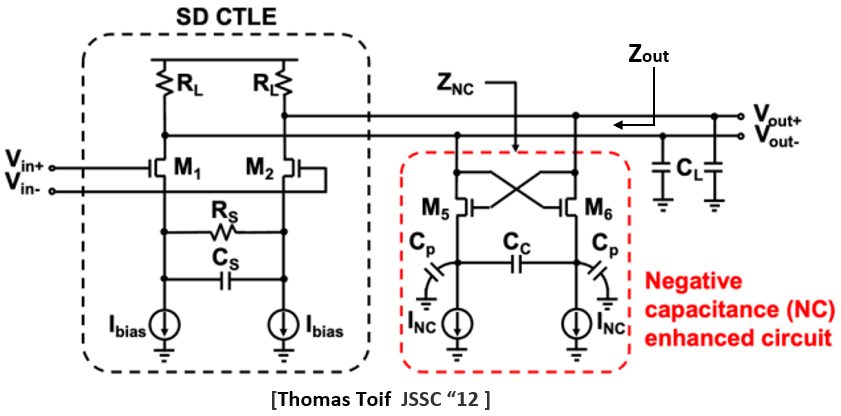
\includegraphics[width=.55\textwidth]{img/CTLE_img/NC SCHEMATIC.png}
    \caption{Negative capacitance CTLE architecture [Thomas Toifl JSSC '12].}
    \label{fig:nc_ctle_schematic}
\end{figure}

The coupling capacitors $C_c$ provide AC coupling, accelerating the positive feedback path by providing low impedance at high frequencies. Near the targeted Nyquist frequency, $C_c$ forms a low impedance, effectively shorting the source terminals of M5 and M6.

\subsubsection*{Negative Impedance Analysis}

The cross-coupled pair (M5, M6) with coupling capacitors $C_c$ creates a negative impedance at the output node. The impedance looking into the negative capacitance circuit can be derived as:

\[
Z_{NC} = -\frac{\frac{1}{sC_C} + \left( \frac{C_{gs5,6}}{C_C} + 2 \right) \frac{1}{g_{m5,6}}}{1 - \frac{sC_{gs5,6}}{g_{m5,6}}}
\]

Near the Nyquist frequency, where $\frac{sC_{gs5,6}}{g_{m5,6}} \ll 1$, this simplifies to:

\[
Z_{NC} = -\frac{1}{sC_C} - \left( \frac{C_{gs5,6}}{C_C} + 2 \right) \frac{1}{g_{m5,6}} = \frac{1}{sC_{NC}} + R_{NC}
\]

where:
\[
\begin{aligned}
C_{NC} &= -C_C, \\
R_{NC} &= -\left(2 + \frac{C_{gs5,6}}{C_C}\right) \cdot \frac{1}{g_{m5,6}}
\end{aligned}
\]

The total output impedance becomes the parallel combination of the load resistance and the negative impedance:

\[
Z_{out} = R_L \parallel Z_{NC} = \frac{R_L \cdot Z_{NC}}{R_L + Z_{NC}}
\]

This parallel combination has a crucial effect: when a negative impedance $Z_{NC}$ is placed in parallel with a positive resistance $R_L$, the magnitude of the total impedance can become larger than $R_L$ alone. This occurs because:

\[
|Z_{total}| = \left| \frac{R_L \cdot Z_{NC}}{R_L + Z_{NC}} \right|
\]

For $R_{NC} < 0$, if $|Z_{NC}| > R_L$, the denominator $R_L + Z_{NC}$ becomes negative with magnitude smaller than $R_L$, resulting in $|R_{total}| > R_L$. This impedance enhancement directly boosts the voltage gain at high frequencies, since: $A_v \propto g_m \cdot |Z_{out}|$

The negative capacitance $C_{NC} = -C_C$ effectively cancels part of the parasitic capacitance at the output node, extending the bandwidth. The combined effect of increased effective resistance and reduced capacitance enables the NC-CTLE to achieve higher gain-bandwidth product compared to conventional SD-CTLE.

\subsubsection{Enhanced Frequency Response Analysis}

\begin{figure}[H]
    \centering
    \begin{minipage}{0.48\textwidth}
        \centering
        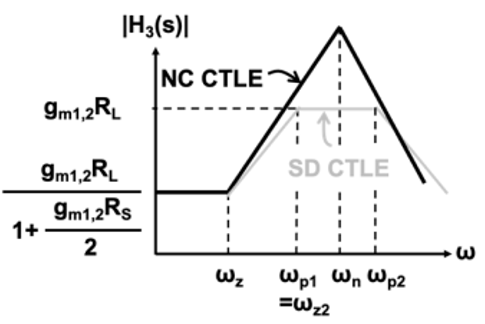
\includegraphics[width=0.7\textwidth]{img/CTLE_img/nc assymptotic response.png}
        \caption{Asymptotic frequency response comparison.}
        \label{fig:nc_asymptotic}
    \end{minipage}
    \hfill
    \begin{minipage}{0.48\textwidth}
        \centering
        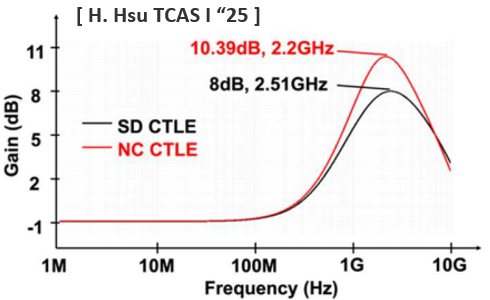
\includegraphics[width=0.7\textwidth]{img/CTLE_img/nc real response .png}
        \caption{Actual response in 180nm technology.}
        \label{fig:nc_real_response}
    \end{minipage}
\end{figure}

The negative capacitance modifies the pole-zero structure while maintaining the same zero $\omega_z$ as SD-CTLE. Assuming $\omega_{p2} \gg \omega_n$ and $\omega_{p2} \gg \omega_{p1}$, the transfer function of the NC-CTLE is derived as:

\[
H_3(s) = -\frac{g_{m1,2}R_L}{1 + \frac{g_{m1,2}R_s}{2}} \cdot \frac{1 + \frac{s}{\omega_z}}{(1 + \frac{s}{\omega_{p1}})(1 + \frac{s}{\omega_n})}
\]

The NC-CTLE introduces a new zero $\omega_{z2}$ and a complex-conjugate pole pair characterized by natural frequency $\omega_n$ and damping factor $\zeta$, where:

\[
\begin{aligned}
\omega_{z2} &= \frac{g_{m5,6}}{2C_C}, &\quad
\omega_n &= \frac{\sqrt{g_{m5,6}}}{\sqrt{2R_LC_LC_C}}, &\quad
\zeta &= \frac{\omega_n}{2} \left( R_LC_L + \frac{2C_L}{g_{m5,6}} - R_LC_C \right)
\end{aligned}
\]

A key design strategy in NC-CTLE is to compensate the first pole $\omega_{p1}$ with the additional zero $\omega_{z2}$, i.e., $\omega_{z2} \approx \omega_{p1}$. This pole-zero cancellation extends the bandwidth by effectively removing the dominant pole limitation. The natural frequency $\omega_n$ then becomes the new dominant frequency that determines the peaking location and magnitude.

The negative capacitance modifies the relationship between $\omega_{p1}$ and $\omega_{p1,NC}$, where $\omega_{p1,NC} < \omega_{p1}$, while $\omega_n > \omega_{p2}$. This modified pole arrangement, shown in Figure~\ref{fig:nc_asymptotic}, creates a wider peaking region and higher maximum gain compared to conventional SD-CTLE. The actual implementation in 180nm technology (Figure~\ref{fig:nc_real_response}) demonstrates NC-CTLE achieving 10.39 dB peaking at 2.2 GHz versus SD-CTLE's 8 dB at 2.51 GHz, representing a 30\% improvement in equalization capability.

\subsubsection{Design Knobs and Tunability}

The NC-CTLE inherits all tuning parameters from the SD-CTLE—$R_L$, $R_s$, $C_s$, and $I_{bias}$ described in Section~\ref{sec:design_knobs}, while introducing the additional critical parameter $I_{NC}$ that controls the negative capacitance strength through $g_{m5,6}$.

\subsubsection*{Effect of Negative Capacitance Current $I_{NC}$}
\label{subsec:effect_inc}

The bias current $I_{NC}$ controls the transconductance $g_{m5,6}$ of the cross-coupled pair (M5, M6), which directly determines the strength of the negative capacitance effect. As shown in Figure~\ref{fig:effect_inc}, increasing $I_{NC}$ from 0.06 mA to 0.16 mA (a 2.67× rise) enhances the peaking gain by 1.9 dB at the cost of a 9.1% reduction in peaking frequency.

\begin{figure}[H]
    \centering
    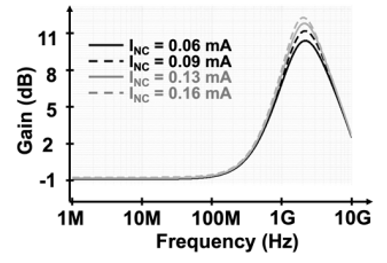
\includegraphics[width=0.5\textwidth]{img/CTLE_img/effect of inc.png}
    \caption{Frequency response variation with increasing $I_{NC}$ from 0.06 mA to 0.16 mA in 180nm technology.}
    \label{fig:effect_inc}
\end{figure}

The mechanism behind this trade-off involves several interconnected effects:

\begin{itemize}
    \item \textbf{Transconductance Increase}: Higher $I_{\text{NC}}$ boosts $g_{m5,6}$, strengthening the positive feedback through the cross-coupled pair.
     
    \item \textbf{Parasitic Capacitance Rise}: The increased $I_{\text{NC}}$ raises parasitic capacitance $C_P$ at the source terminals of M5 and M6.
     
    \item \textbf{Zero Frequency Modification}: The additional zero $\omega_{z2}$ is revised to:
    \[
    \omega_{z2} \approx \frac{g_{m5,6}}{2C_C} \rightarrow \frac{g_{m5,6}}{2C_C + C_P'}
    \]
    With higher $C_P$, $\omega_{z2}$ decreases.
     
    \item \textbf{Natural Frequency Reduction}: The natural frequency also decreases due to the larger $C_P$:
    \[
    \omega_n = \sqrt{\frac{g_{m5,6}}{2R_L C_L C_C}} \rightarrow \sqrt{\frac{g_{m5,6}}{2R_L C_L (C_C + C_P/2)}}
    \]
    contributing to lower peaking frequency.
     
    \item \textbf{Damping Factor Reduction}: A critical side effect of increasing $I_{\text{NC}}$ is the reduction in damping factor $\zeta$, given by:
    \[
    \zeta = \frac{\omega_n}{2} \left( R_L C_L + \frac{2C_L}{g_{m5,6}} - R_L \left( C_C + \frac{C_P}{2} \right) \right)
    \]
    Lower $\zeta$ increases the risk of under-damping, causing ringing in the time-domain response and potential eye diagram degradation.
\end{itemize}

When $\omega_{z2} < \omega_{p1}$, the gain increases with a steeper slope before encountering $\omega_{p1}$, thereby boosting the peaking gain. This explains the gain improvement with increasing $I_{\text{NC}}$. However, the accompanying reduction in $\zeta$ necessitates careful design to avoid excessive peaking and eye diagram closure, especially under PVT variations.

\newpage
\subsubsection*{Damping Factor and Stability Considerations}
\label{subsec:damping_stability}

The damping factor $\zeta$ is critical for NC-CTLE stability and time-domain performance. As derived from the transfer function and noted in the circuit analysis, $\zeta$ is given by:
\[
\zeta = \frac{\omega_n}{2} \left( R_LC_L + \frac{2C_L}{g_{m5,6}} - R_L \left( C_C + \frac{C_P}{2} \right) \right)
\]
where $\omega_n = \sqrt{\frac{g_{m5,6}}{2R_L C_L (C_C + C_P/2)}}$ is the natural frequency, and $C_P$ is the parasitic capacitance at the source terminals of M5 and M6. Increasing $I_{\text{NC}}$ raises $g_{m5,6}$ but also $C_P$, which can significantly reduce $\zeta$, leading to under-damping and potential instability.

\begin{figure}[H]
    \centering
    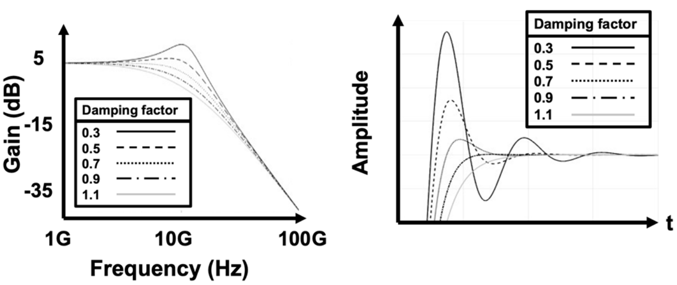
\includegraphics[width=0.85\textwidth]{img/CTLE_img/nc damping factor.png}
    \caption{Impact of damping factor $\zeta$ on frequency response (top) and step response (bottom). Lower $\zeta$ increases peaking and introduces ringing.}
    \label{fig:nc_damping}
\end{figure}

Figure~\ref{fig:nc_damping} illustrates the effect of $\zeta$ on both frequency and time-domain responses:

\begin{itemize}
    \item \textbf{High $\zeta$ ($>1$)}: Over-damped response with insufficient peaking, resulting in reduced bandwidth and smaller eye openings.
    \item \textbf{Optimal $\zeta$ ($0.7$–$1.0$)}: Provides adequate peaking for channel compensation without excessive ringing, maximizing eye height and timing margin.
    \item \textbf{Low $\zeta$ ($<0.5$)}: Under-damped behavior causing significant overshoot, ringing, and potential eye diagram closure.
\end{itemize}

\newpage
\subsubsection*{PVT Variations and Design Margins}

The NC-CTLE exhibits significant sensitivity to process, voltage, and temperature (PVT) variations, primarily because $\zeta$ depends directly on $g_{m5,6}$, which varies with $I_{\text{NC}}$ and transistor characteristics.

\begin{figure}[H]
    \centering
    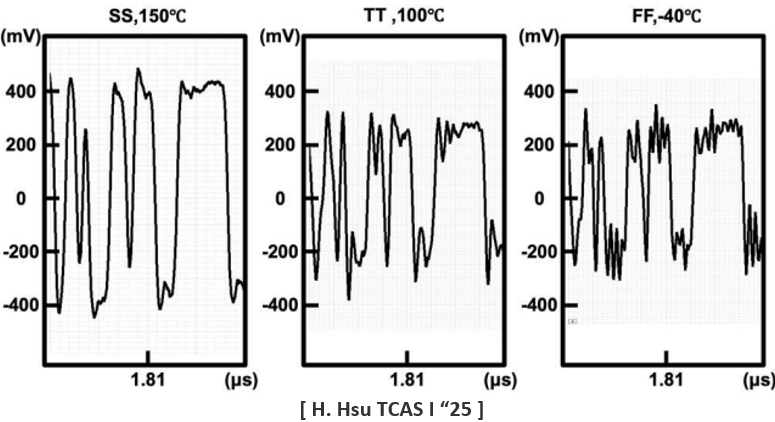
\includegraphics[width=0.85\textwidth]{img/CTLE_img/pvt variations.png}
    \caption{PVT variations affecting NC-CTLE response across process corners and temperatures [H. Hsu TCAS I '25].}
    \label{fig:pvt_variations}
\end{figure}

As shown in Figure~\ref{fig:pvt_variations}, the impact of PVT corners includes:

\begin{itemize}
    \item \textbf{Fast-Fast (FF) Corner at Low Temperature}: Higher $g_{m5,6}$ reduces $\zeta$, causing noticeable ringing and potential eye degradation.
    \item \textbf{Slow-Slow (SS) Corner at High Temperature}: Reduced $g_m$ decreases negative capacitance effect and peaking magnitude, possibly under-equalizing the channel.
    \item \textbf{Temperature Effects}: Higher temperatures generally reduce $g_m$, diminishing the negative capacitance enhancement and shifting $\zeta$ upward.
\end{itemize}

To ensure reliable operation across all corners, the following design practices are recommended:

\begin{enumerate}
    \item Design $\zeta$ with sufficient margin above the minimum stable value at nominal conditions, typically targeting $\zeta_{\text{nominal}} \geq 1.0$.
    \item Implement a tunable $I_{\text{NC}}$ range to compensate for $g_m$ variations across PVT.
    \item Consider on-die temperature compensation or calibration loops in high-performance applications.
    \item Co-optimize $C_C$, $R_L$, and $I_{\text{bias}}$ to reduce sensitivity to $C_P$ variations.
\end{enumerate}

\subsubsection*{Eye Diagram Performance and Risks}

\begin{figure}[H]
    \centering
    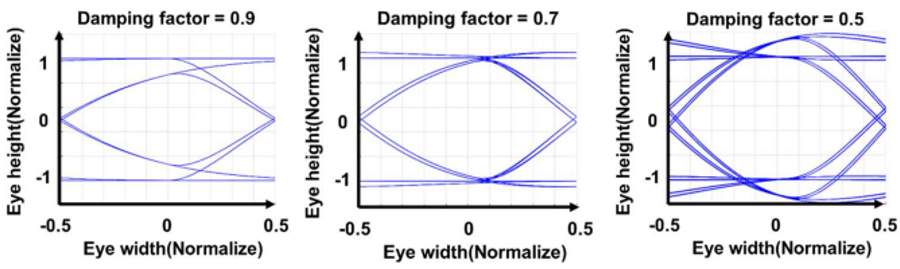
\includegraphics[width=\textwidth]{img/CTLE_img/nc eye diagram.png}
    \caption{Eye diagram variation with damping factor $\zeta$. Lower $\zeta$ increases peaking but introduces ISI and jitter from ringing.}
    \label{fig:nc_eye_diagram}
\end{figure}

The enhanced peaking of NC-CTLE improves eye diagrams for severely lossy channels but introduces stability-related risks, as shown in Figure~\ref{fig:nc_eye_diagram}:

\begin{itemize}
    \item \textbf{Optimal $\zeta$ Range}: Delivers significantly improved eye height and width compared to SD-CTLE, effectively compensating for channel loss.
    \item \textbf{Low $\zeta$ Risk}: Excessive peaking causes ringing in the time domain, reducing timing margin, increasing jitter, and potentially closing the eye.
    \item \textbf{High $\zeta$ Limitation}: Over-damped response fails to provide sufficient high-frequency boost, leaving residual ISI.
    \item \textbf{Practical Implementation}: NC-CTLE offers higher peaking gain than SD-CTLE but at the cost of reduced peaking frequency and increased sensitivity to $I_{\text{NC}}$ tuning.
\end{itemize}

\subsubsection{Design Trade-offs and Guidelines}

\begin{table}[H]
\centering
\caption{Design Trade-offs for Negative Capacitance CTLE}
\label{tab:nc_ctle_tradeoffs}
\begin{tabular}{ >{\raggedright\arraybackslash}p{0.15\textwidth} 
                 >{\raggedright\arraybackslash}p{0.23\textwidth} 
                 >{\raggedright\arraybackslash}p{0.25\textwidth} 
                 >{\raggedright\arraybackslash}p{0.30\textwidth} }
\toprule
\textbf{Parameter} & \textbf{Benefit} & \textbf{Risk} & \textbf{Design Guideline} \\
\midrule
$I_{\text{NC}}$ & Higher peaking gain & Lower $\zeta$, stability risk & Adaptive control, monitor $\zeta$ \\
\midrule
$g_{m5,6}$ & Stronger negative capacitance & PVT sensitivity, higher $C_P$ & Temperature compensation, margin design \\
\midrule
$\zeta$ & Guarantees stability & Reduced peaking if too high & Target $\zeta \approx 0.8$–$1.0$ with PVT margin \\
\midrule
$C_C$ & HF feedback coupling & Bandwidth limit with $C_P$ & Co-design with $C_P$ in frequency planning \\
\midrule
$C_P$ & N/A (parasitic) & Reduces $\omega_n$ and $\zeta$ & Minimize layout parasitics, account in simulation \\
\bottomrule
\end{tabular}
\end{table}